\renewcommand{\thechapter}{3}
\chapter{The EXO-200 Detector}
\label{ch:EXO200Detector}

This chapter describes the physical apparatus of the EXO-200 detector.  Section~\ref{sec:DetectorOverview} gives a broad overview of the detector.  Section~\ref{sec:DetectorBackgrounds} identifies the dominant backgrounds for $\beta\beta 0\nu$ decay, and sections~\ref{sec:DetectorPassiveBackgroundRejection} and \ref{sec:DetectorActiveBackgroundRejection} describe methods used to mitigate these backgrounds.  The pulse and waveform readout subsystems are described in section~\ref{sec:DetectorReadout}, where discussion of the scintillation readout will be particularly important for subsequent chapters.  We conclude with a description of the calibration systems in section~\ref{sec:DetectorCalibration}.  Throughout, the reader is referred to the detailed description in~\cite{detectorPartI} for more information.

\section{Overview of the EXO-200 Detector}\label{sec:DetectorOverview}

The EXO-200 detector is a cryogenic experiment containing $175$ kg of liquid xenon enriched to $80.6\%$ in $^{136}$Xe.  Of those $175$ kg of liquid xenon, $110$ kg are contained within the ``active'' volume where the detector is fully sensitive to deposited energy from $\beta\beta 0\nu$ decay~\cite{detectorPartI}, and $94.7$ kg are contained within the fiducial volume where the detector's response is well-understood.  This implies that $3.39 \cdot 10^{26}$ atoms $^{136}$Xe which are for the search~\cite{NewEXObb0nPaper_2014}.

\begin{figure}
\begin{center}
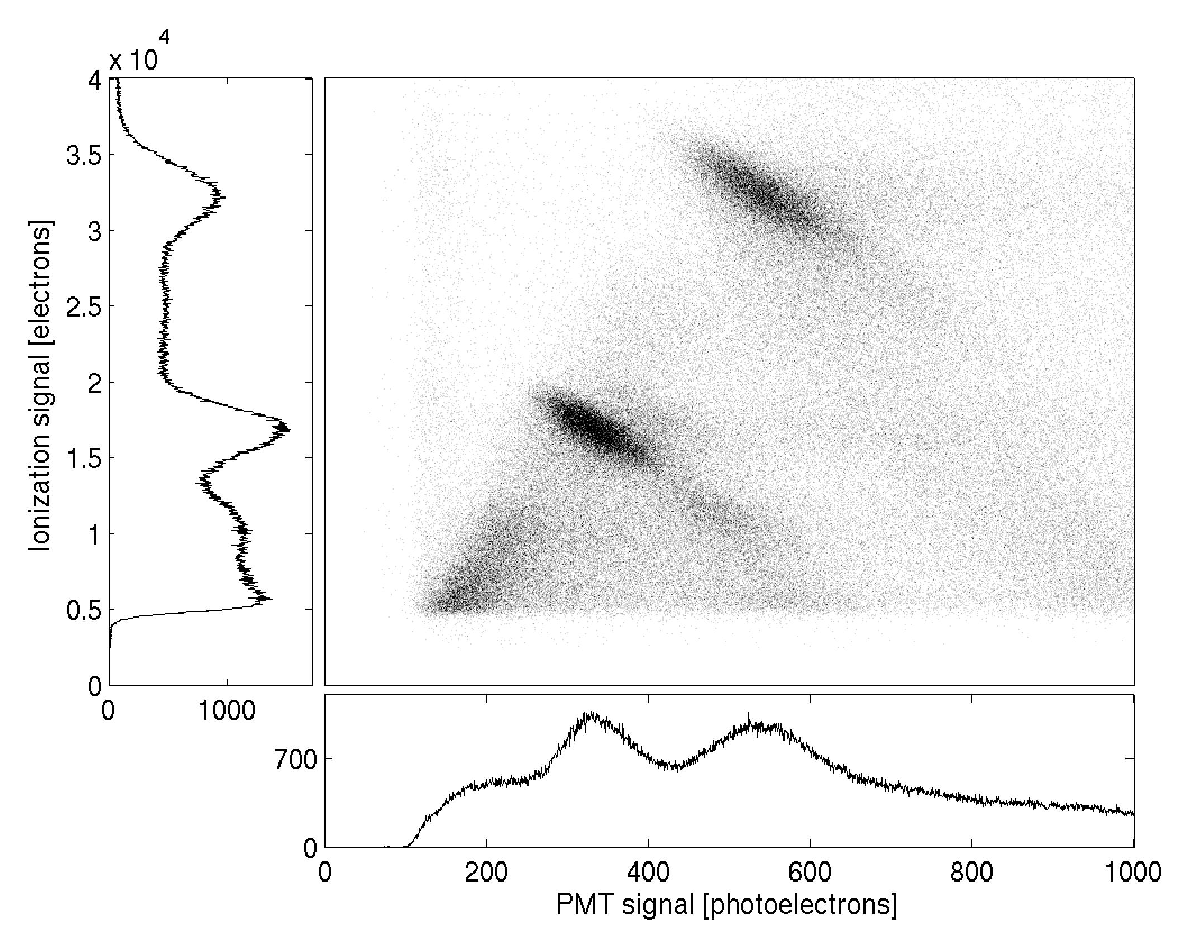
\includegraphics[keepaspectratio=true,width=\textwidth]{4kV_correl1.eps}
\end{center}
\renewcommand{\baselinestretch}{1}
\small\normalsize
\begin{quote}
\caption{A two-dimensional energy spectrum of scintillation and ionization from a testbed liquid xenon experiment under an electric field of $4$ kV/cm.  The spectrum is from a $^{207}$Bi source with dominant gamma lines at 570 and 1064 keV.  Figure reproduced from~\cite{PhysRevB.68.054201}.}
\label{fig:AnticorrelationInXenon}
\end{quote}
\end{figure}
\renewcommand{\baselinestretch}{2}
\small\normalsize

Energy deposits in xenon can be measured primarily in two ways: vacuum ultraviolet (VUV) scintillation photons are emitted from the de-excitation of xenon eximers, and xenon atoms are ionized to produce free electrons.  It is well-known~\cite{PhysRevB.68.054201} that liquid noble element calorimeters show significant fluctuations in their separate production of scintillation photons and free electrons, but that these separate quantities are strongly anticorrelated.  As a result, it is possible to achieve far better energy resolution if both light and charge are independently measured than if only one is detected. Figure~\ref{fig:AnticorrelationInXenon} illustrates this phenomenon in a testbed liquid xenon experiment, where it is apparent that using light and charge simultaneously lets us observe narrower gamma lines than either would individually; the same is also true of beta and double-beta lines such as the $\beta\beta 0\nu$ decay we seek.

\begin{figure}
\begin{center}
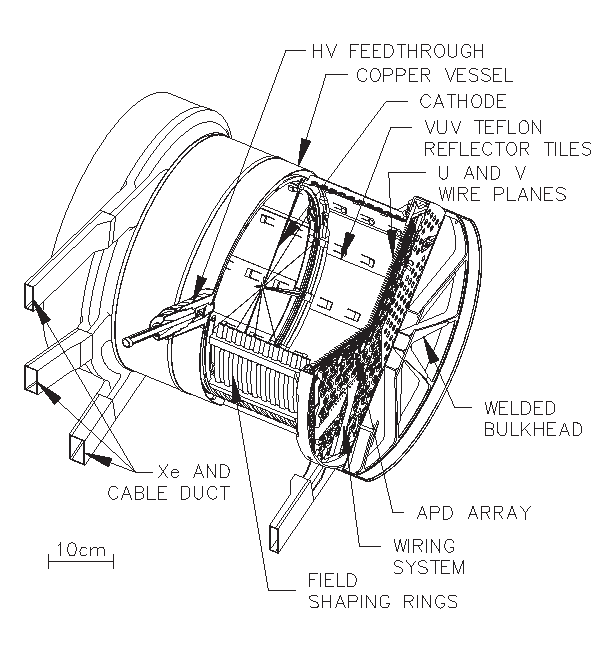
\includegraphics[keepaspectratio=true,width=\textwidth]{TPCSchematic.eps}
\end{center}
\renewcommand{\baselinestretch}{1}
\small\normalsize
\begin{quote}
\caption{Schematic of the inner EXO-200 TPC.  Figure reproduced from~\cite{detectorPartI}.}
\label{fig:TPCSchematic}
\end{quote}
\end{figure}
\renewcommand{\baselinestretch}{2}
\small\normalsize

To observe free electrons we must impose an electric field on the xenon which drifts the electrons onto a collection anode.  The EXO-200 detector is shaped as a cylinder, and the required electric field is produced by placing a cathode grid in the center of that cylinder and anode wires along each of the two endcaps of the detector; such a detector is called a time projection chamber, or TPC.  The EXO TPC is shown in figure~\ref{fig:TPCSchematic}.  Charge is collected on the anode wires and light is collected by avalanche photo-diodes (see section~\ref{sec:DetectorReadout}) mounted on the endcaps behind the anode wires; the time difference between the two signals indicates the initial position of the charge along the direction of the field. The anode wires are thin, so the u- and v-wire planes together have 91.8\% optical transparency which does not interfere significantly with APD light collection~\cite{detectorPartI}.

The cathode is maintained at a voltage of $-8$ kV below the anode wire voltage, which is at virtual ground.  Field shaping rings encircle the charge drift region to ensure that electric field lines are parallel and the magnitude of the electric field is constant in the bulk volume of xenon.  (Near the edges, non-uniformities in the electric field are expected to exist; these are a continuing topic of research.)  The cathode and APDs are separated by $20.4$ cm. The bulk volume of xenon has an electric field of $374$ V/cm.

Electrons in liquid xenon drift at a velocity of $1.71$ mm/$\mu$s under an electric field of $374$ V/cm.  The maximum drift distance from the cathode to the anode is $198.4$ mm, resulting in a maximum electron drift time of $116$ $\mu$s.  Free electrons are not absorbed by xenon -- as for other noble elements, xenon has a low electronegativity, so in pure xenon electrons drift unimpeded indefinitely.  The EXO-200 liquid xenon has small quantities of electronegative impurities which could include oxygen or nitrogen.  The exact nature of these impurities is unknown.  To minimize the concentration of these impurities, the xenon is constantly circulated through a hot zirconium getter which extracts chemically active molecules and permits noble elements to pass through~\cite{detectorPartI}.

It is necessary to associate charge pulses with their corresponding scintillation pulses because they are separated by an unknown drift time of up to 116 $\mu$s.  This is easily done provided the typical time between events is much longer than $116$ $\mu$s, and the time difference serves as our measurement of the position of the energy deposit along the direction of the electric field.  Our 1 $\mu$s sampling rate permits us to reconstruct this position coordinate with an accuracy of $0.42$ mm~\cite{bb2nEXO2014}.

\begin{figure}
\begin{center}
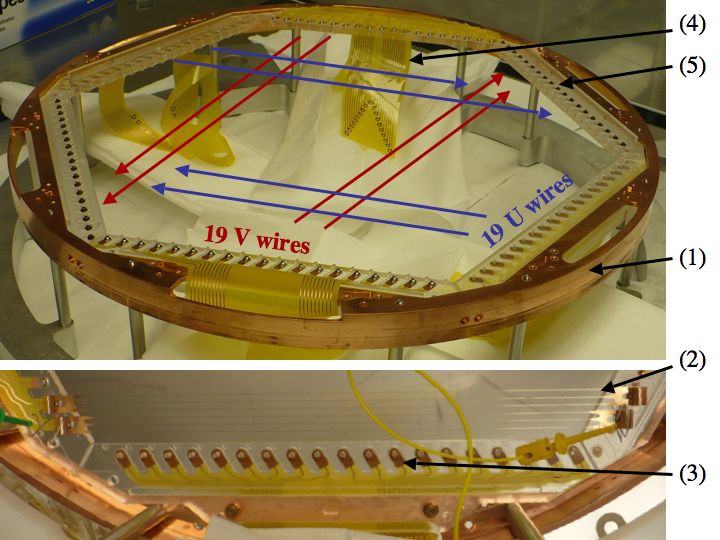
\includegraphics[keepaspectratio=true,width=\textwidth]{supportwithoutwires.png}
\end{center}
\renewcommand{\baselinestretch}{1}
\small\normalsize
\begin{quote}
\caption{Anode collection wires (u-wires) and induction wires (v-wires) from EXO-200.  (1) and (5) indicate the wire support frame; (2) indicates the wires themselves, constructed as gangs of three wires; (3) illustrates the attachment between wires and the support frame; (4) shows the return cables from the wires to the data acquisition system.  Figure reproduced from~\cite{detectorPartI}.}
\label{fig:UandVWiresCrossing}
\end{quote}
\end{figure}
\renewcommand{\baselinestretch}{2}
\small\normalsize

At the anode, there are two sets of parallel wire planes as shown in figure~\ref{fig:UandVWiresCrossing}.  The first (closer to the cathode) parallel wire plane is called the ``v-wire'' plane, and the second plane is called the ``u-wire'' plane.  The voltages of the two wire planes are set so that no drift field lines terminate on the v-wires. Instead, all drift field lines penetrate through the v-wire plane and terminate on the u-wires.  When charge is deposited in the liquid xenon and drifts toward the anode, it induces a bipolar current on the v-wires as it passes by, and then produces a unipolar current on the u-wires as it is collected.  See section~\ref{sec:DetectorReadout} for details on the wire readout and section~\ref{sec:ResultsDigitization} for illustrations of the expected pulse shapes.

The u- and v-wires are rotated sixty degrees relative to each other.  Figure~\ref{fig:UandVWiresCrossing} indicates the orientation of the u-wires and v-wires, and figure~\ref{fig:FidVolDiagram} illustrates from top-down perspective the u-v coordinate system defined by the wires alongside the x-y coordinate system used in analysis.  By detecting which wires observe a current pulse in both the u-wire and v-wire channels, it is possible to identify the two-dimensional location on the anode where the charge arrived.  Channels in each plane are $9$ mm wide; by taking advantage of signal sharing which sometimes occurs between u-wires and always occurs between v-wires, we are able to achieve position accuracy of $2.4$ mm perpendicular to the u-wires and $1.2$ mm perpendicular to the v-wires~\cite{bb2nEXO2014}.

Energy which appears to come from a single location is called a charge deposit ``cluster'' or ``site'', and events are classified according to the number of sites they produce (their ``multiplicity'') as either single-site or multi-site.  We will see in section~\ref{sec:DetectorActiveBackgroundRejection} that this provides a powerful tool for background characterization and rejection.

This section has described how energy deposits in the liquid xenon are transformed into scintillation and charge, which are then observed by APDs and anode wires, respectively.  These observations are sufficient for us to reconstruct the positions and magnitudes of energy deposits in the liquid xenon in all three coordinates.

\section{Backgrounds to \texorpdfstring{$\beta\beta 0\nu$}{Neutrinoless Double-Beta} Decay}\label{sec:DetectorBackgrounds}

$^{136}$Xe has a relatively high $Q$-value compared to $^{76}$Ge; in the neutrinoless mode the two emitted electrons will share $2456.7$ keV~\cite{NewEXObb0nPaper_2014}.  This means that the sensitivity of $T_{1/2}^{0\nu}$ to the mass of the neutrino is good in $^{136}$Xe compared to $^{76}$Ge, as was described in section~\ref{sec:NucPhysConstraintsFromBB0N}; it also means that the energy spectrum around our $Q$-value will naturally be relatively free from most sources of background radiation.  This section will identify the types of background which can be expected to affect our $\beta\beta 0\nu$ search; subsequent sections will describe methods of mitigating those backgrounds.

It is common for alpha decays to have energies well in excess of our $Q$-value.  As a result, we might expect all alpha decays to be possible backgrounds to $\beta\beta 0\nu$.  However, alpha particles are stopped rapidly by even a small quantity of shielding, and as a result the only alpha decays which can be observed in the detector are those from sources which are dissolved into the xenon.  Radon is the only alpha-emitting noble element, and in EXO-200 only $^{222}$Rn is sufficiently long-lived to diffuse into the xenon; as a result, we only expect $^{222}$Rn and its daughter products to contribute a significant quantity of alpha decays to the detector.

Cosmic rays produce high-energy muons; these are another source of high-energy backgrounds.  Observations using the EXO-200 detector have indicated that the vertical flux of muons $\Phi_v$ is
\begin{equation}
\Phi_v =  \left(4.01 \pm 0.04(\mathrm{stat}){}^{+0.04}_{-0.05} (\mathrm{sys})\right) \times 10^{-7} \frac{\mathrm{Hz}}{\mathrm{cm}^2 \mathrm{sr}}
\end{equation}
which implies a depth of $1481^{+8}_{-6}$ meters water-equivalent~\cite{ThesisSteve}.  The depth and muon flux of WIPP relative to other underground facilities can be seen in figure~\ref{fig:MuonFluxVsDepth}.  Muons which pass through the TPC will produce a streak of energy in the detector rather than discrete clusters; generally they will have sufficient energy to pass fully through the detector.  We can expect that such an event will look substantially different from a $\beta\beta 0\nu$ event, and generally will deposit substantially more energy than our $Q$-value as well.

More interesting are the associated by-products from the nearby passage of such a high-energy particle through the EXO-200 shielding or the surrounding salt, called spallation products.  Although high-energy muons can produce a range of fission products, the most significant spallation product of muons will be neutrons which can diffuse into the detector and activate materials there.  $^{134}$Xe and $^{136}$Xe are both present in significant quantities in the TPC, and by activation can be converted into the radioactive isotopes $^{135}$Xe and $^{137}$Xe respectively.  $^{135}$Xe has an endpoint decay energy of 1165 keV which is too small for it to be a background to $\beta\beta 0\nu$ decay, but $^{137}$Xe undergoes $\beta$ decay with an endpoint energy of $4173$ keV.  We will see that indeed $^{137}$Xe is a significant source of background in our detector~\cite{NewEXObb0nPaper_2014,NeutronCaptureGammas}.

Some sources of background are intrinsic to the $\beta\beta 0\nu$ search.  Any isotope which can undergo $\beta\beta 0\nu$ decay can also undergo $\beta\beta 2\nu$ decay, and the endpoint of the $^{136}$Xe $\beta\beta 2\nu$ spectrum is necessarily at our $Q$-value.  The only means of reducing background from $\beta\beta 2\nu$ is to improve the energy resolution of the detector so that fewer such decays can mimic $\beta\beta 0\nu$ decay.  Fortunately with the energy resolution exhibited by the EXO-200 detector, $\beta\beta 2\nu$ is subdominant to other backgrounds by many orders of magnitude~\cite{NewEXObb0nPaper_2014}.

Similarly, it is hypothetically possible for neutrino absorption to stimulate a single-$\beta$ decay which would otherwise have been energetically forbidden; that isotope may then undergo a second single-$\beta$ decay with a $Q$-value greater than the $Q$-value of the $\beta\beta 0\nu$ decay, acting as a background for our search.  For example, in $^{136}$Xe the reaction $^{136}\mathrm{Xe} + \nu_e \rightarrow ^{136}\mathrm{Cs} + \mathrm{gammas}$ can occur; $^{136}$Cs will then undergo single-$\beta$ decay with an endpoint energy of 2548 keV and half-life of 13.6 days.  This energy is above the $Q$-value for $^{136}$Xe $\beta\beta 0\nu$ decay.  However, this process is expected to occur at quite a low rate, and estimates indicate that it will be a negligible background until $^{136}$Xe sensitivities reach $T_{1/2}^{0\nu} \approx 10^{27}$ years~\cite{0954-3899-30-9-R01,1309.7957}.

\begin{figure}
\begin{center}
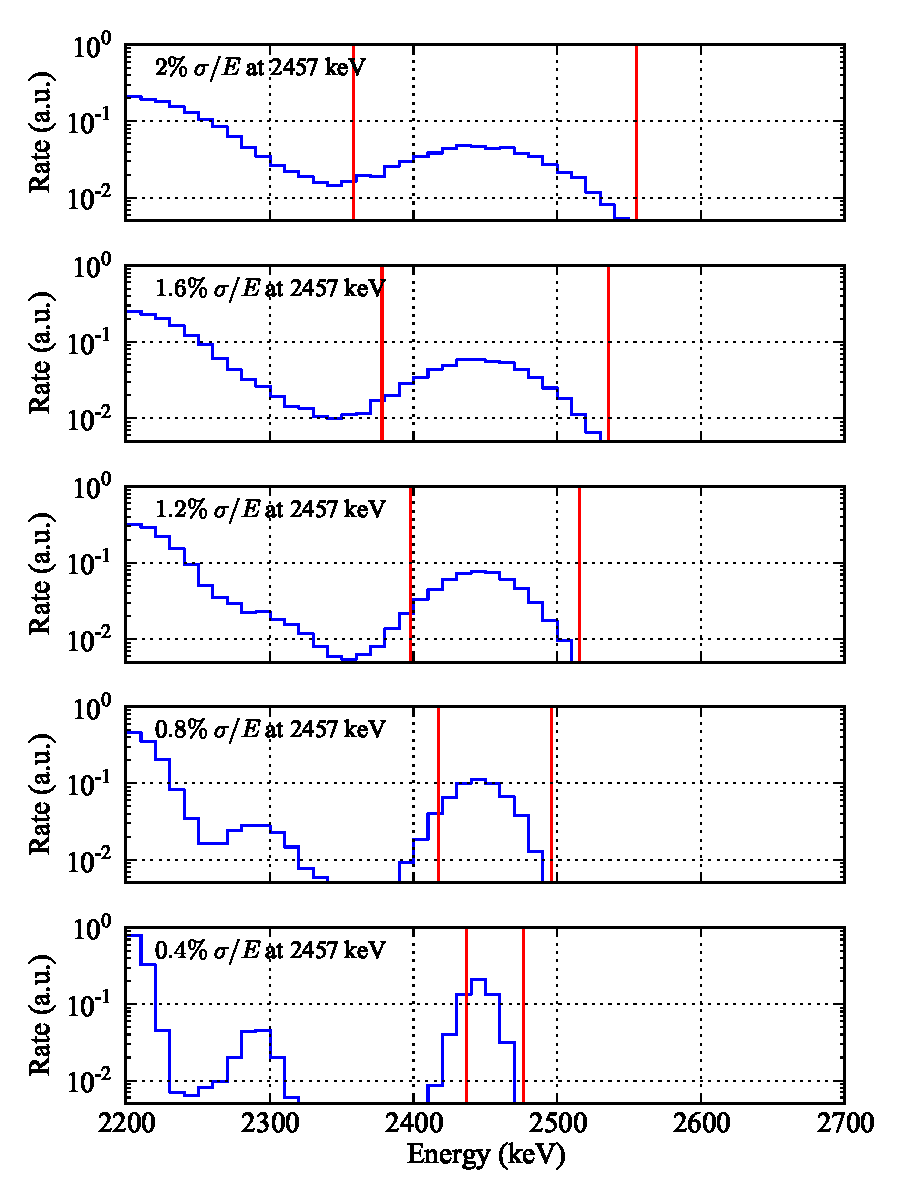
\includegraphics[keepaspectratio=true,width=.92\textwidth]{scripts/U_Spectra_vs_Res.pdf}
\end{center}
\renewcommand{\baselinestretch}{1}
\small\normalsize
\begin{quote}
\caption{Representative $^{238}$U spectra as the energy resolution of the detector changes.  Red lines indicate the $2\sigma$ region of interest around the $Q$-value.  Normalization is arbitrary, but all spectra have the same normalization.  Betas and gammas are assumed to have the same calibration here; alternative beta scales are considered in section~\ref{sec:ResultFitting}.}
\label{fig:USpectraVsResolution}
\end{quote}
\end{figure}
\renewcommand{\baselinestretch}{2}
\small\normalsize

A gamma background which is particularly detrimental to EXO-200 comes from $^{214}$Bi, a member of the $^{226}$Ra decay chain.  $^{214}$Bi emits a gamma at $2448$ keV with a branching ratio of $1.548\%$, which with our energy resolution is indistinguishable from our $Q$-value.   $^{226}$Ra has a half-life of $1600$ years and generally will be supported by $^{230}$Th ($75,000$ years), $^{234}$U ($250,000$ years), and ultimately by $^{238}$U ($4.5 \cdot 10^9$ years) which has a primordial abundance in the Earth's crust and most natural materials~\cite{ENSDF}.  Figure~\ref{fig:USpectraVsResolution} shows the $^{238}$U energy spectrum as the energy resolution improves; we can see that even with excellent resolution the 2448 keV gamma line will be a problematic $\beta\beta 0\nu$ background.

\begin{figure}
\begin{center}
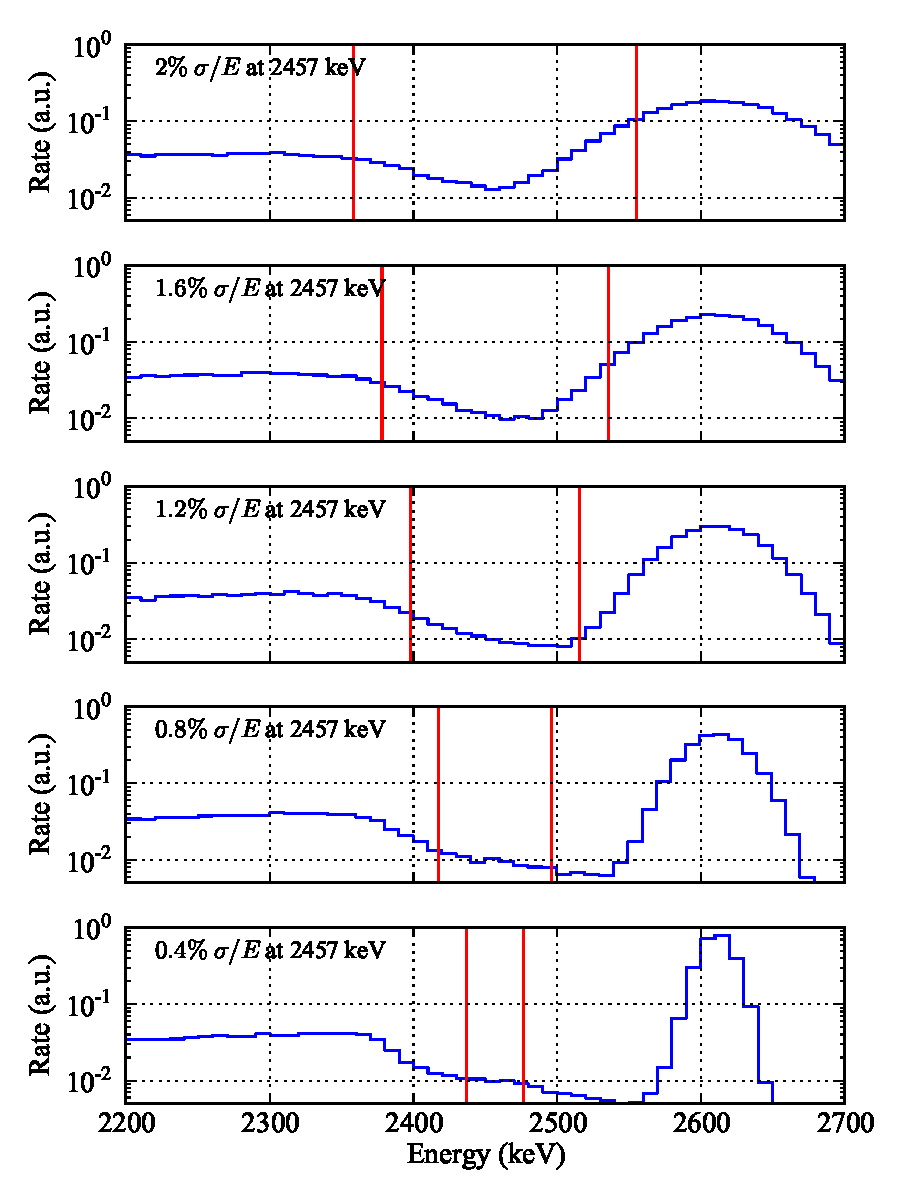
\includegraphics[keepaspectratio=true,width=.92\textwidth]{scripts/Th_Spectra_vs_Res.pdf}
\end{center}
\renewcommand{\baselinestretch}{1}
\small\normalsize
\begin{quote}
\caption{Representative $^{232}$Th spectra as the energy resolution of the detector changes.  Red lines indicate the $2\sigma$ region of interest around the $Q$-value.  Normalization is arbitrary, but all spectra have the same normalization.  Betas and gammas are assumed to have the same calibration here; alternative beta scales are considered in section~\ref{sec:ResultFitting}.}
\label{fig:ThSpectraVsResolution}
\end{quote}
\end{figure}
\renewcommand{\baselinestretch}{2}
\small\normalsize

Most other backgrounds to $\beta\beta 0\nu$ will be gamma decays from $^{208}$Tl, a member of the $^{232}$Th decay chain.  $^{208}$Tl is produced from $^{232}$Th with a $35.94\%$ branching ratio and emits a gamma at $2614.5$ keV with a $99.74\%$ branching ratio; with our $Q$-value of $2456.7$ keV, the two energies are separated by $157.8$ keV~\cite{ENSDF}.  The energy resolution (in $\sigma/E$ at our $Q$-value) of EXO-200 has historically been $1.5-2\%$ at these energies~\cite{NewEXObb0nPaper_2014}, meaning that separation between the central values of the gamma lines will be $3-4\sigma$.  (If betas and gammas have different calibrations then this number may vary; see section~\ref{sec:ResultFitting} for more information on the beta scale.)  $^{232}$Th has a half-life of $14$ billion years and a significant abundance in most natural materials; we expect it to contribute a significant fraction of our radioactive backgrounds, and as a result some events from the $2615$ keV $^{208}$Tl line will leak across those $3-4\sigma$ and act as backgrounds.  Improving the energy resolution to $1.5\%$ will reduce contamination from this gamma line.

The Compton edge is a well-known feature of gamma scattering spectra; it originates from gammas which enter a calorimeter, scatter once, and escape from the detector.  The maximum energy which a gamma of incident energy $E_{inc}$ can deposit in a single scatter is:~\cite{Compton}
\begin{equation}
E_{dep} = \frac{2E_{inc}^2}{m_e c^2 + 2E_{inc}}.
\end{equation}
When the incident gamma has an energy of $2615$ keV, the Compton edge will lie at $2382$ keV, or only $74.5$ keV below our $Q$-value.  If our energy resolution is around $1.5-2\%$ $\sigma/E$ at these energies, this separation is $1.5-2\sigma$.  At energy resolutions which are better than about $1.4\%$, we find that the Compton edge begins to contribute more background to our $2\sigma$ region of interest than the gamma line at 2615 keV; we can see this phenomenon from the energy spectra of figure~\ref{fig:ThSpectraVsResolution}.

\begin{figure}
\begin{center}
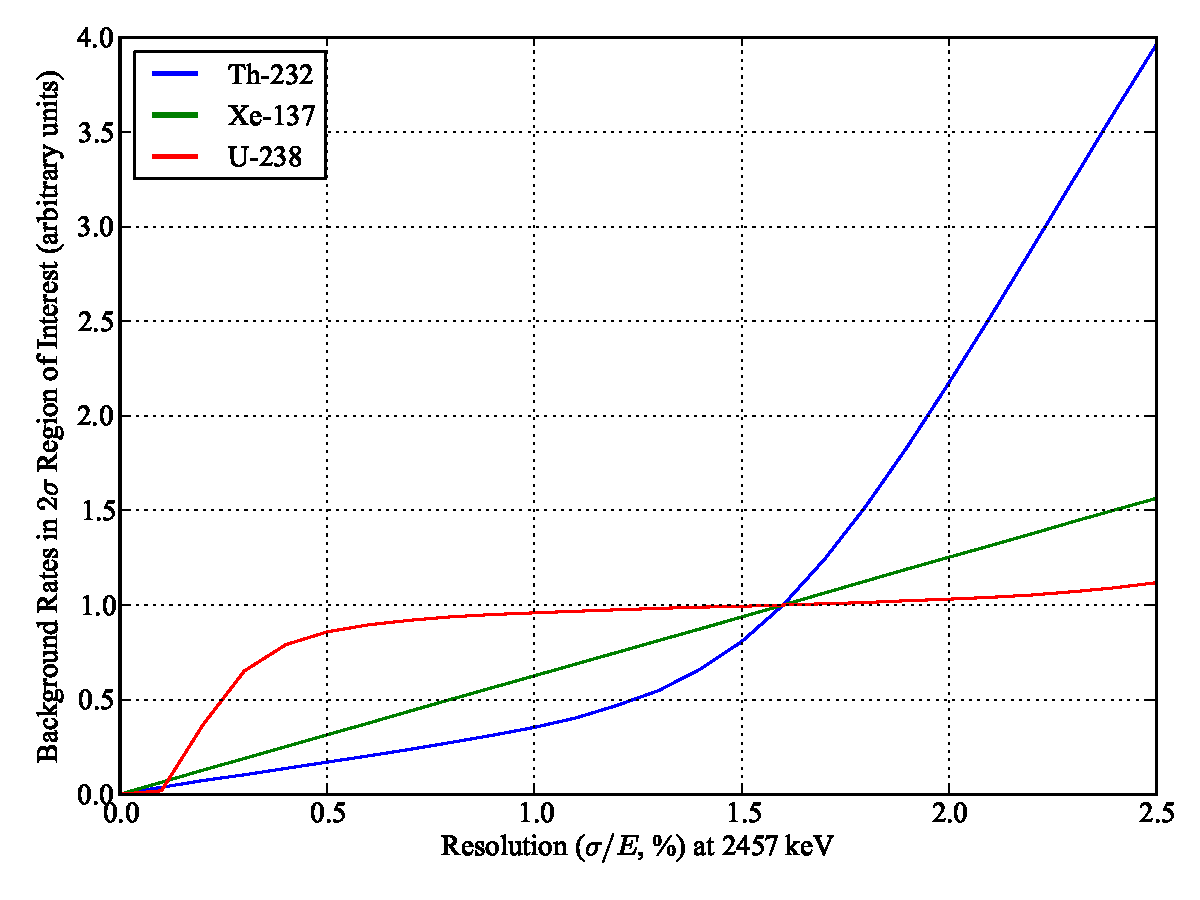
\includegraphics[keepaspectratio=true,width=\textwidth]{scripts/BackgroundsVsRes.pdf}
\end{center}
\renewcommand{\baselinestretch}{1}
\small\normalsize
\begin{quote}
\caption{Relative change in background rates expected in our $2\sigma$ region of interest as a function of the energy resolution.  Rates are normalized to one at a $Q$-value energy resolution of $1.6\%$ $\sigma/E$, the design goal of EXO-200.  The three backgrounds shown, from $^{232}$Th, $^{238}$U, and $^{137}$Xe, are currently our dominant backgrounds.  Betas and gammas are assumed to have the same calibration here; alternative beta scales are considered in section~\ref{sec:ResultFitting}.}
\label{fig:BackgroundVsResolution}
\end{quote}
\end{figure}
\renewcommand{\baselinestretch}{2}
\small\normalsize

Figure~\ref{fig:BackgroundVsResolution} summarizes the background rates from our three dominant backgrounds, $^{232}$Th, $^{238}$U, and $^{137}$Xe, as they depend on the energy resolution of the detector.  We can see that the background rates of $^{232}$Th and $^{238}$U do not vary smoothly with resolution due to the presence of gamma lines; by contrast, the spectrum of $^{137}$Xe is smooth and its background rates decrease linearly with resolution.  The EXO-200 detector has a time-averaged resolution of $1.94\%$ $\sigma/E$ without the denoising technique described in this work, and $1.53\%$ $\sigma/E$ with denoising; we can see that this results in a significant reduction of backgrounds from $^{232}$Th.  However, improvements in resolution will not decrease the backgrounds from $^{238}$U unless resolutions below $0.5\%$ $\sigma/E$ are reached, which is not feasible with the current detector.  The following sections will identify some of the mechanisms beyond energy resolution which are used to further minimize these backgrounds.

\section{Passive Background Rejection}\label{sec:DetectorPassiveBackgroundRejection}

We can distinguish between two classes of background rejection methods: passive methods, in which backgrounds are reduced by reducing the amount of background reaching the liquid xenon, and active methods, in which backgrounds are observed by the detector but discriminated from $\beta\beta 0\nu$ signal based on identifying characteristics.  In this section, passive methods will be described; section~\ref{sec:DetectorActiveBackgroundRejection} will describe the active methods of background rejection.  The passive methods we will identify are exploiting the self-shielding properties of xenon, screening the materials for radioactivity, and putting the experiment deep underground.

\begin{figure}
\begin{center}
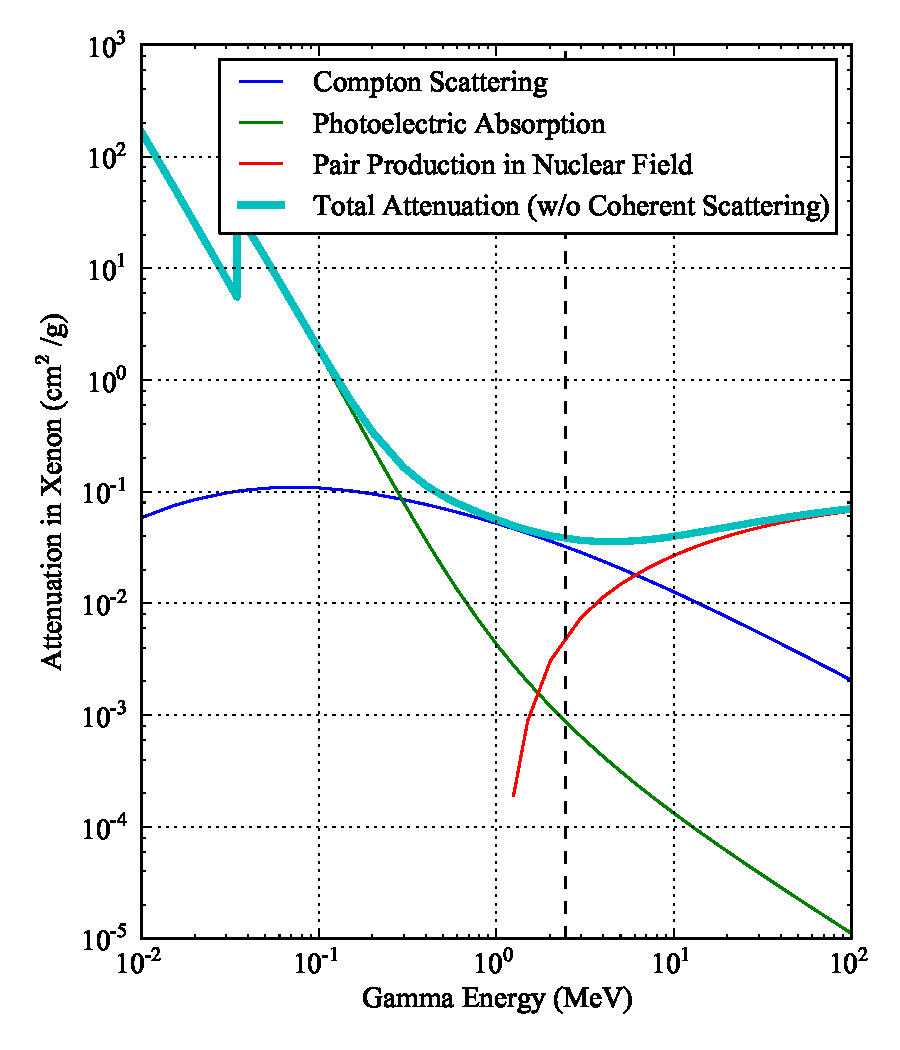
\includegraphics[keepaspectratio=true,width=\textwidth]{scripts/XrayAttenuationXenon.pdf}
\end{center}
\renewcommand{\baselinestretch}{1}
\small\normalsize
\begin{quote}
\caption{X-ray attenuation lengths in xenon.  Compton scattering, pair production, and photoelectric absorption are shown, along with their combined attenuation length; coherent (Rayleigh) scattering is omitted because it produces no observable energy deposit.  The $Q$-value of $^{136}$Xe $\beta\beta 0\nu$ decay is indicated with a dashed black line.  The vertical axis, in $\text{cm}^2/\text{g}$, can be multiplied by the density of the xenon to derive an attenuation factor per unit length.  Data from~\cite{XcomXenonAttenuation}.}
\label{fig:XrayAttenuationXenon}
\end{quote}
\end{figure}
\renewcommand{\baselinestretch}{2}
\small\normalsize

The simplest method of reducing the presence of backgrounds is by exploiting the self-shielding properties of xenon.  The xenon itself is extremely pure due to the ease of chemical purification.  As a result most backgrounds will be external to the xenon.  Since external gammas are weakly attenuated by dense materials such as liquid xenon, which has a density of $3.0305 \pm 0.0077$ g/cm$^3$~\cite{bb2nEXO2014}, we can expect that the xenon near the center of the detector will be exposed to less background than the xenon near the TPC walls.  This is one of the primary advantages of xenon as a source: it is possible to construct a large monolithic detector, maximizing the quantity of xenon which is shielded from the walls.

Figure~\ref{fig:XrayAttenuationXenon} shows the attenuation lengths of gammas at a range of energies in xenon.  Photoabsorption and pair production both convert the gamma entirely into short-ranged electron and positron carriers; Compton (incoherent) scattering results in a fractional energy deposition, with the rest remaining in the gamma which rebounds and continues on a deflected path.  Enriched liquid xenon has a density of $3.0305 \pm 0.0077$ g/cm$^3$~\cite{bb2nEXO2014}, which means that the minimal attenuation factor is $0.108/\text{cm}$ at an energy of $4.34$ MeV.  Unfortunately, this is similar to our $Q$-value at $2456.7$ keV, where the attenuation factor is still only $0.116/\text{cm}$, which means that self-shielding is minimally effective for $\beta\beta 0\nu$.  Nevertheless, there is some reduction in backgrounds deeper in the interior of the xenon, and lower-energy gammas are attenuated more effectively~\cite{XcomXenonAttenuation}.

To reduce the quantity of background around the detector, all materials near the xenon were carefully screened for radioactive contamination~\cite{MaterialsCatalog}.  Backgrounds from $^{40}$K, $^{232}$Th, and $^{238}$U were cataloged for all materials which have unshielded line-of-sight access to the detector system.  Requirements for $^{238}$U are particularly stringent because its daughter products include the $^{214}$Bi background which cannot be resolved from $\beta\beta 0\nu$ decay.  For the copper of the TPC vessel and the lead shielding around the detector apparatus, samples from a range of companies and mines were tested to locate an optimal choice of material source.  For the wires which were placed into the TPC, a range of manufacturing methods were tested; improvements to a photo-etching scheme were identified which led to a reduction in background from these materials~\cite{detectorPartI}.  This thorough material screening research is one of the distinctive processes which has enabled EXO-200 to achieve its background goals.  Details of the quantification of and constraints on material radioactivity can be found in~\cite{MaterialsCatalog}.

Beyond selecting extremely clean materials, it is possible to reduce backgrounds by minimizing the mass of these external materials.  Most notably, the EXO-200 copper TPC vessel is, in most places, only $1.37$ mm thick. To maintain structural integrity, supporting structures are welded to the TPC where needed. The total mass of copper is less than $30$ kg~\cite{detectorPartI}.

Some materials were dispensed with entirely.  Typically, silicon APDs are encapsulated with ceramic to isolate them from water contamination and provide electrical insulation.  However, this ceramic material would have contributed backgrounds.  Instead, the APDs were delivered ``bare,'' without any encapsulation, and protected from water by storing them in a dry-nitrogen container.  Liquid xenon itself serves as an electrical insulator, ensuring the APDs would function properly during detector operations~\cite{EXOLAAPD}.

\begin{figure}
\begin{center}
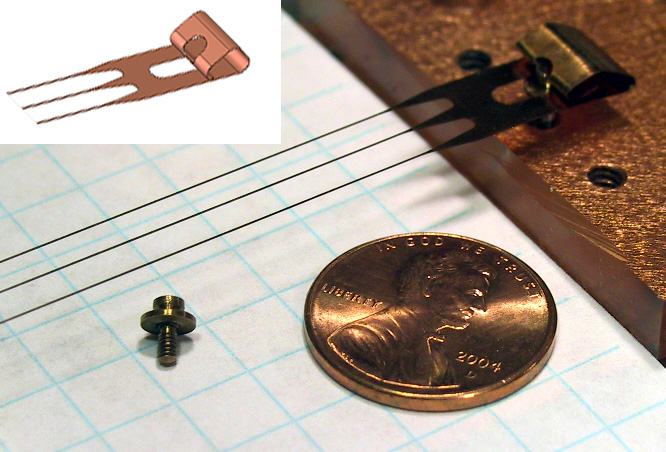
\includegraphics[keepaspectratio=true,width=\textwidth]{triplet.jpg}
\end{center}
\renewcommand{\baselinestretch}{1}
\small\normalsize
\begin{quote}
\caption{Wire triplet, read as one channel.  Figure from~\cite{detectorPartI}.}
\label{fig:WireTriplet}
\end{quote}
\end{figure}
\renewcommand{\baselinestretch}{2}
\small\normalsize

\begin{figure}
\begin{center}
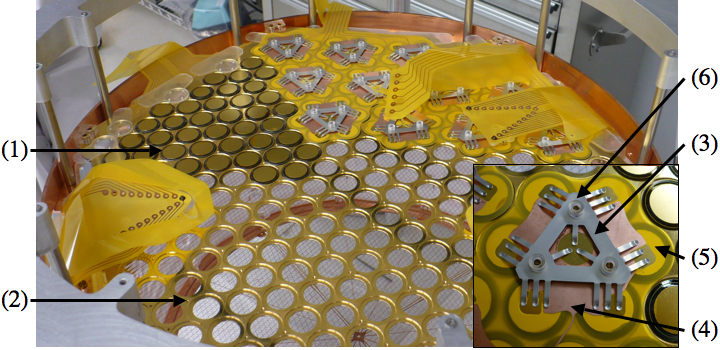
\includegraphics[keepaspectratio=true,width=\textwidth]{PlatterWGO7.png}
\end{center}
\renewcommand{\baselinestretch}{1}
\small\normalsize
\begin{quote}
\caption{APDs ganged together (bottom right).  Wiring to the front-end electronics are visible as yellow ``tape.''  Figure from~\cite{detectorPartI}.}
\label{fig:APDgang}
\end{quote}
\end{figure}
\renewcommand{\baselinestretch}{2}
\small\normalsize

The cabling of the wires and APDs was also done with great care.  The electrical amplifiers and digitizers contain many high-background plastics, metals, and other complex materials, so they were placed outside the lead shielding rather than close to the TPC.  Wires connect the sensors in the TPC to these electronics; ordinarily such long wires would need to be shielded by coaxial cabling to minimize cross-talk noise.  However, the coaxial cabling was expected to contribute a high quantity of radioactive background, and was omitted; instead wires are partially electrically shielded by surrounding them with inactive wires which reduce cross-talk noise.  Furthermore, the total number of wires needed was reduced by ganging together triplets of u- and v-wires and groups of six or seven APDs into single channels. This reduced the fineness of event information available in analysis, but also reduced the quantity and complexity of material placed near the detector.  The wire gangs are shown in figure~\ref{fig:WireTriplet}; APD gangs cabling are visible in figure~\ref{fig:APDgang}~\cite{detectorPartI}.

\begin{figure}
\begin{center}
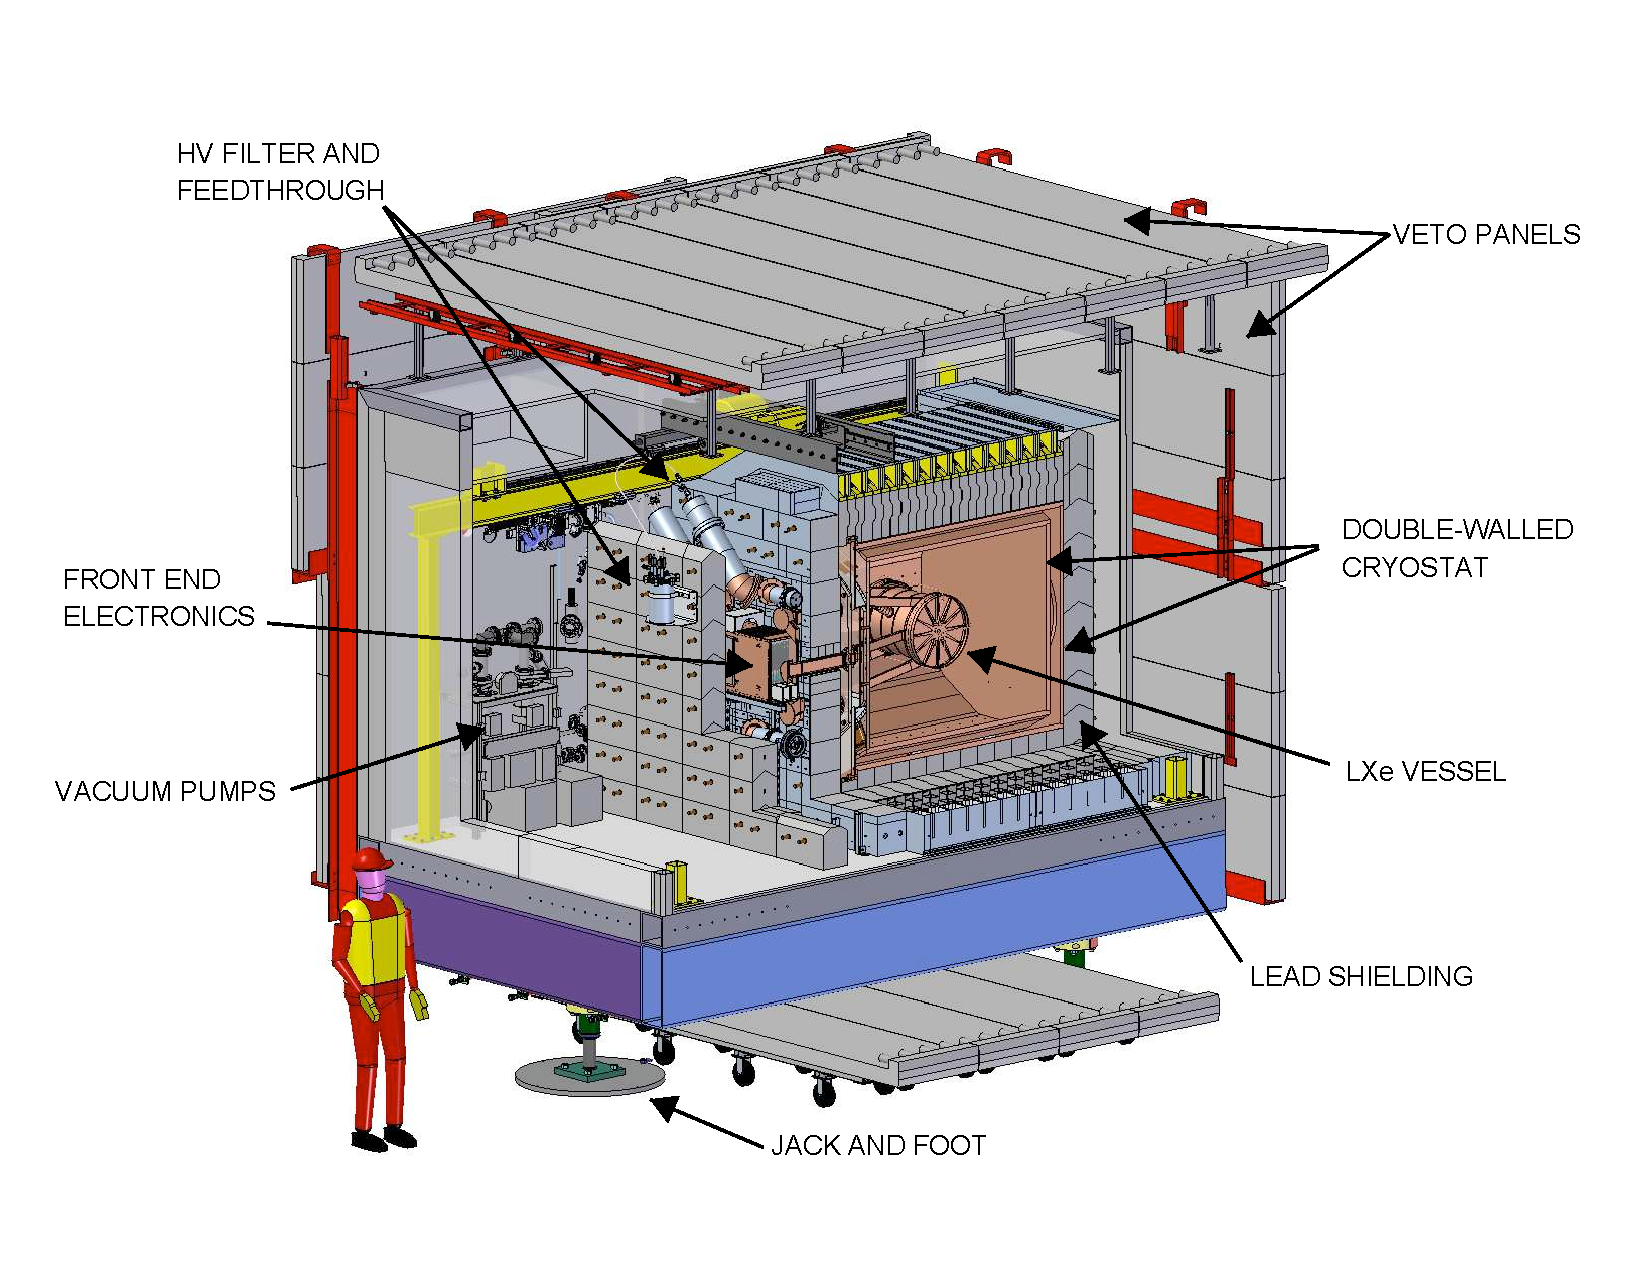
\includegraphics[keepaspectratio=true,width=\textwidth]{cleanroom.pdf}
\end{center}
\renewcommand{\baselinestretch}{1}
\small\normalsize
\begin{quote}
\caption{A cutaway schematic image of the TPC and surrounding materials in the cleanroom.  HFE-7000 refrigerant is contained between the cryostat and the LXe vessel.  Figure from~\cite{detectorPartI}.}
\label{fig:CleanRoomCutaway}
\end{quote}
\end{figure}
\renewcommand{\baselinestretch}{2}
\small\normalsize

The TPC is shielded by nested layers of clean material designed to prevent backgrounds from reaching the xenon.  In the innermost layer, HFE-7000 refrigerant (see figure~\ref{fig:CleanRoomCutaway}) is used to maintain the detector at liquid xenon temperatures and to shield from external gammas.  However, the HFE-7000 has a significant quantity of hydrogen, which also makes it an excellent stopping agent for thermal neutrons.  The refrigerant layer is more than $50$ cm thick, so most external neutrons thermalize, absorb onto hydrogen, and emit a 2.2 MeV gamma rather than reaching the TPC and producing $^{137}$Xe with its more harmful 4173 keV beta endpoint energy~\cite{detectorPartI}.

The following layer of shielding is copper cryostat, then lead, shown in figure~\ref{fig:CleanRoomCutaway}.  This is a common approach for low-background experiments due to the high density of lead, which enables it to stop gammas in a short distance.  Lead bricks surround the detector on all sides; the bricks were designed with an interlocking shape to ensure no seams between bricks left a line-of-sight path from external sources into the TPC.  In the front of the detector, where plumbing must enter and exit the detector through the first lead wall, a second lead wall is assembled with the purpose of blocking any line-of-sight paths into the TPC through the plumbing gaps of the first wall~\cite{detectorPartI}.

\begin{figure}
\begin{center}
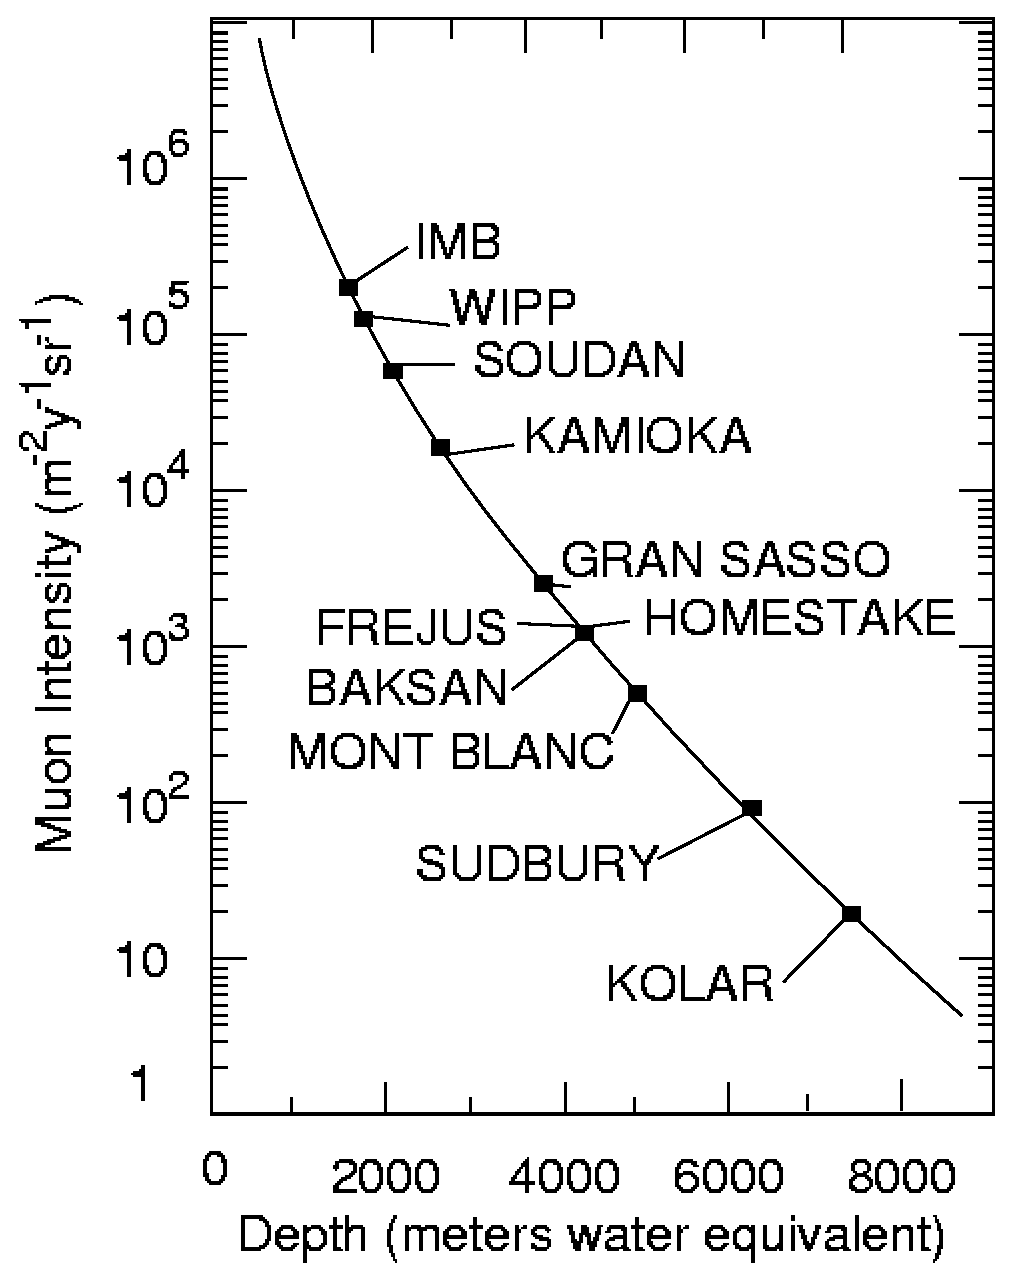
\includegraphics[keepaspectratio=true,width=\textwidth]{muonflux.eps}
\end{center}
\renewcommand{\baselinestretch}{1}
\small\normalsize
\begin{quote}
\caption{Muon flux as a function of depth, in meters water equivalent.  The WIPP site is indicated in relation to other underground science facilities.  Figure from~\cite{Esch2005516}.}
\label{fig:MuonFluxVsDepth}
\end{quote}
\end{figure}
\renewcommand{\baselinestretch}{2}
\small\normalsize

Outside of the lead shielding, restrictions on materials are less stringent; however, control over the presence of materials is still desired.  The entire apparatus is contained inside a class-1000 cleanroom facility.  The entire facility is located in the Waste Isolation Pilot Plant (WIPP) facility, a Department of Energy waste repository located in a salt formation near Carlsbad, NM.  The overburden of the facility is $1481^{+8}_{-6}$ meters water-equivalent~\cite{ThesisSteve}.  Figure~\ref{fig:MuonFluxVsDepth} shows the reduction in muon flux due to depth at the WIPP site and a selection of other underground science facilities.

These passive approaches have all been demonstrated to reduce the rate of backgrounds depositing energy in the liquid xenon.  The following section will describe an active set of background-rejection approaches.

\section{Active Background Rejection}\label{sec:DetectorActiveBackgroundRejection}

This section will describe the ``active'' forms of background reduction employed by the EXO-200 detector, in which events are observed but discriminated from $\beta\beta 0\nu$ events based on their characteristics.  We neglect the energy resolution as a background rejection tool here, since section~\ref{sec:DetectorBackgrounds} has already described how the impact of certain backgrounds may be reduced by improvement to the energy resolution.

A number of cosmogenic backgrounds have been described: neutrons and fission products can be produced from muons penetrating down to the depth of the WIPP facility.  To reject many of these events, it is sufficient to detect the passage of a muon anywhere near the detector.  This is accomplished by a set of plastic scintillator veto panels surrounding the cleanroom on four of six sides.  Muons are detected by coincident PMT hits on opposite sides of a single panel, with $(96.0 \pm 0.5)\%$ efficiency for detecting muons which traverse the TPC~\cite{detectorPartI}.  Further reduction in the impact of muon-induced backgrounds is achieved by searching for muon tracks observed within the TPC itself, and also by applying a one-second coincident event cut as a catch-all for spallation products of muons which may decay multiple times in rapid succession.

Alpha decays within the xenon are another possible source of high-energy backgrounds.  However, it is possible to discriminate alpha decays from beta and gamma decays based on the properties of their energy measurement.  Alphas produce a far more dense energy deposit in liquid xenon than betas and gammas; the dense collection of free electrons and ionized xenon has a higher rate of charge recombination than is observed with betas and gammas, which translates into a higher ratio of scintillation to ionization for alphas than for betas and gammas.  This feature can be used to eliminate essentially all alpha backgrounds.

Discriminating between gamma, beta, and double-beta decays is more difficult.  Betas from external backgrounds will not penetrate into the xenon due to their short attenuation lengths, so only dissolved beta emitters are backgrounds to $\beta\beta 0\nu$ decay; this constrains the number of plausible beta decays that must be considered.  Gammas generally deposit their energy by ionizing atomic electrons of xenon, so in this way their behavior closely mimics that of betas.  However, most gammas within our energy window (and particularly gammas near our $Q$-value) will be attenuated by Compton (incoherent) scattering, as can be seen in figure~\ref{fig:XrayAttenuationXenon}.  By this process the gamma will deposit energy in more than one discrete location, which beta and double-beta decay will not do.  We are generally able to resolve the positions of these energy deposits and classify the event as multi-site. More than half of external gamma backgrounds are classified as multi-site, whereas the fraction of $\beta\beta 0\nu$ events classified as multi-site due to bremsstrahlung is only $5\%$~\cite{bb2nEXO2014}.

Finally, the liquid xenon itself is continuously purified and quite low in backgrounds, so most radioactive backgrounds in EXO-200 are external.  We have noted that 94.7 kg of liquid xenon are treated as fiducial; the remaining quantity of roughly 15 kg of xenon which is in the active volume of the detector is used as an active veto shield, where any interaction which deposits energy in this volume disqualifies the entire event from use as a $\beta\beta 0\nu$ candidate.  Moreover, the fits which will be described in section~\ref{sec:ResultFitting} take into account the depth into the detector of an energetic deposit, giving events near the exterior greater likelihood of being an external background than events deep inside the xenon.  These strategies give us some discriminating power against external backgrounds.

These are some of the basic techniques employed to reduce backgrounds in offline analysis, and the detector has been designed with the goal of facilitating their application.  The EXO-200 detector currently has two and a half years of data with enriched xenon, and although improvements to the passive methods of background reduction cannot be applied to this existing dataset, it may be hoped that these active methods may be improved or extended through further analysis.  These improvements could have the potential to reduce backgrounds below their current levels in offline analysis, making them a particularly attractive target now that EXO-200 has collected a significant dataset.

\section{Pulse Amplification and Waveform Readout}\label{sec:DetectorReadout}

\begin{figure}
\begin{center}
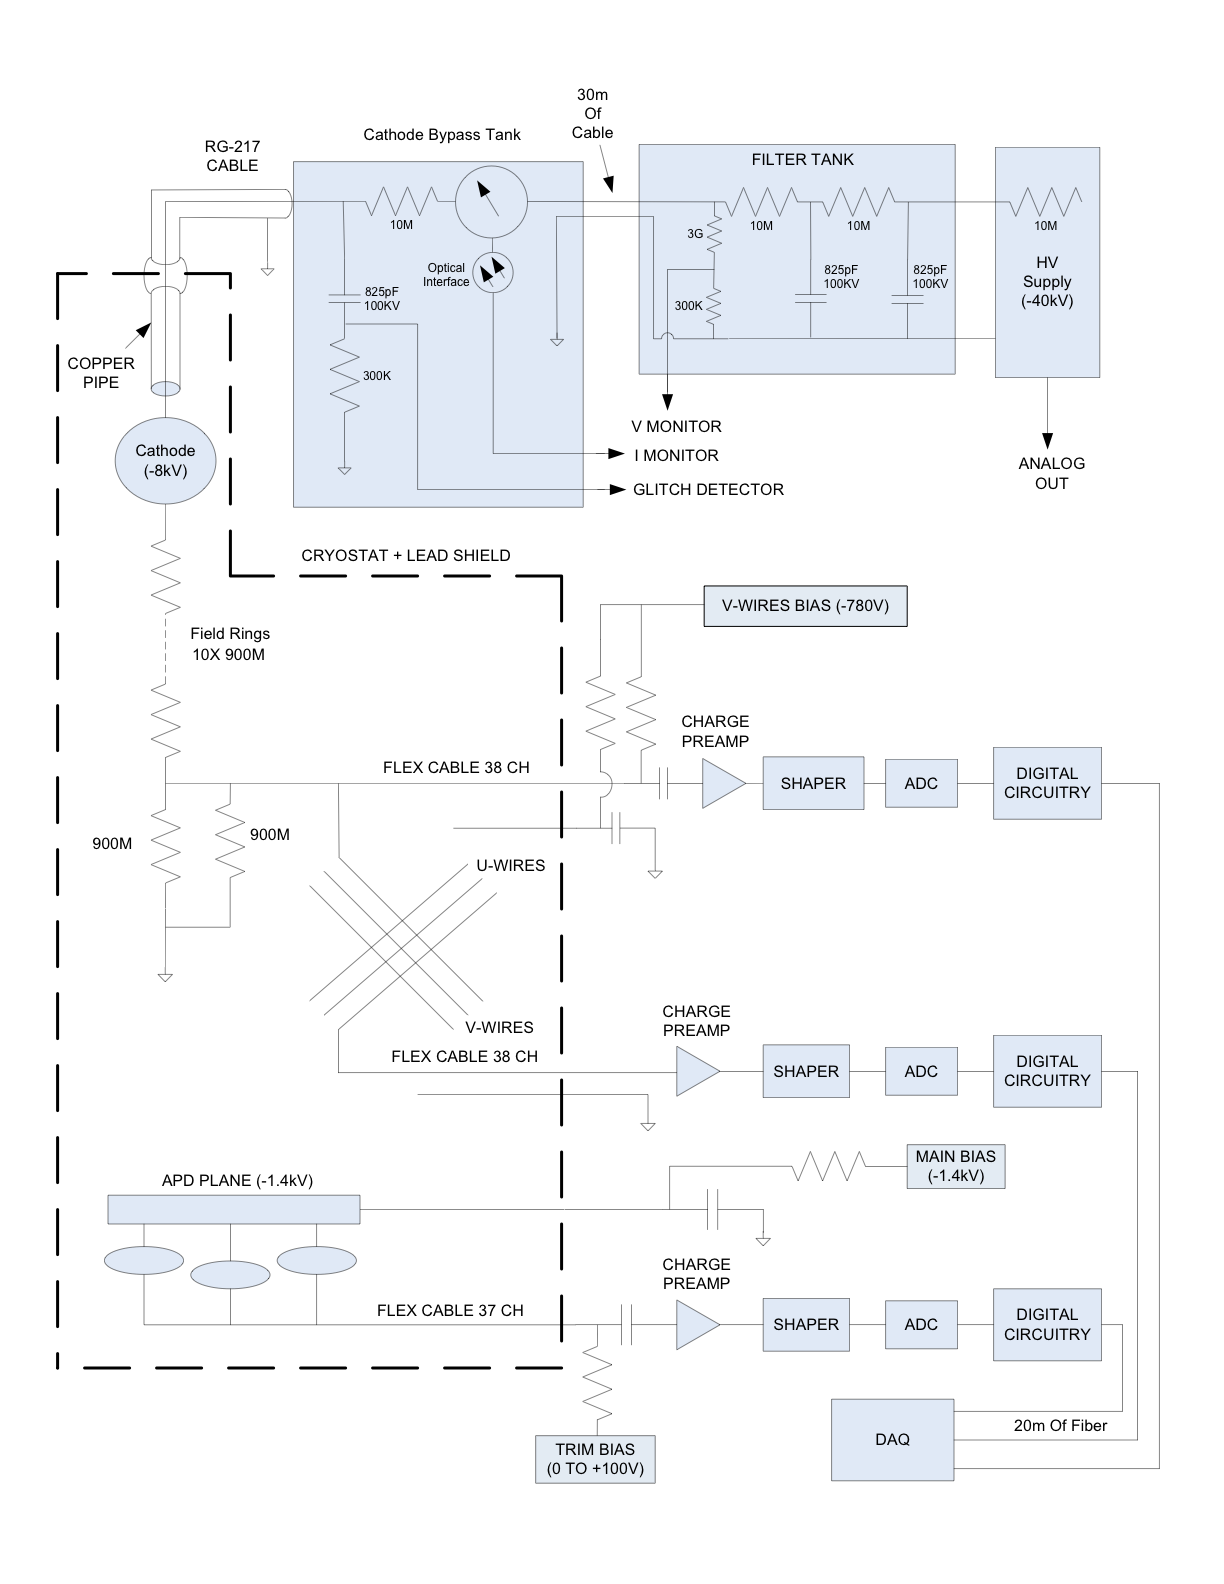
\includegraphics[keepaspectratio=true,width=\textwidth]{FrontEndElectronicsSchematic.png}
\end{center}
\renewcommand{\baselinestretch}{1}
\small\normalsize
\begin{quote}
\caption{An overview of the EXO-200 electronics and readout subsystems.  The area inside the dashed line indicates cold subsystems inside the cryostat or TPC.  Figure from~\cite{detectorPartI}.}
\label{fig:ElectronicsAndReadoutSchematic}
\end{quote}
\end{figure}
\renewcommand{\baselinestretch}{2}
\small\normalsize

This section will provide a brief overview of the EXO electronics and waveform readout.  Particular attention is paid to subsystems which are relevant to the denoising algorithm described in chapter~\ref{ch:DenoisingTheory}, including the APDs and front-end electronics.  A schematic of the electronics and readout subsystems can be seen in figure~\ref{fig:ElectronicsAndReadoutSchematic}.

\begin{figure}
\begin{center}
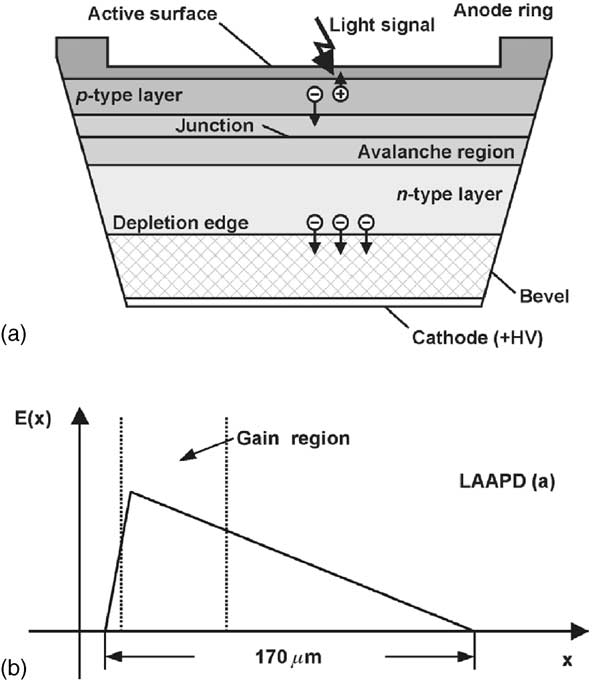
\includegraphics[keepaspectratio=true,width=\textwidth]{APDCrossSection.png}
\end{center}
\renewcommand{\baselinestretch}{1}
\small\normalsize
\begin{quote}
\caption{A cross-sectional schematic of an APD is shown in (a).  The electric field as a function of depth is shown in (b).  Figure from~\cite{Moszynski2002504}.}
\label{fig:APDCrossSection}
\end{quote}
\end{figure}
\renewcommand{\baselinestretch}{2}
\small\normalsize

The APDs are constructed from a silicon semiconductor which is doped and biased so that:~\cite{Moszynski2002504}
\begin{enumerate}
\item Photons arriving at the active surface of the APD can deposit their energy by generating an electron-hole pair in the silicon semiconductor.
\item The electron-hole pair is drifted apart by an electric field.  Here the electric field is low and the silicon is doped to be of p-type (electron-poor), ensuring a similar number of electron-hole pairs are produced by all photons before any amplification can occur.
\item The electron enters a high-field n-type (electron-rich) region of silicon, and liberates additional electron-hole pairs in an avalanche effect.
\item Electrons reach another p-type region of silicon, and then are collected on a cathode as an output current pulse.
\end{enumerate}
These phases of the APD are illustrated in figure~\ref{fig:APDCrossSection}.

$851$ APDs were specially made for EXO-200; from those, $468$ were selected for use based on their favorable noise and gain properties ~\cite{EXOLAAPD}.  For each APD, the relative quantum efficiency and the bias voltage needed to ensure the product of gain and quantum efficiency equals one hundred were both measured.  APDs were assigned to gangs and pies so that their products of gain and quantum efficiency could be set to one hundred as uniformly as possible ~\cite{APDMeasurementAndGanging}.  It is impossible to make the gain of all APDs perfectly uniform because of limitations in the configurability of the APD bias voltages in EXO-200 ~\cite{detectorPartI}.  We note that the current operating conditions of EXO-200 establish a higher operating gain of around $200-300$. This may have the side effect of making the product of gain and quantum efficiency less uniform in each APD gang.

In the u-wires, charge is collected and delivered directly to the electronics as current.  In the v-wires, no net charge is delivered, but transient currents are induced in such a way that the v-wire remains at a constant voltage; these transient currents produce a bipolar pulse, such that the integral (before shaping) is zero.  We note that the pulse shape depends on the drift path of ionization in the liquid xenon -- both sets of wires deliver a current signal which is induced from approaching charge before the charge deposits on the u-wires, and the path of the electrons can affect the time development and, in the case of the v-wires, the magnitude of that induced current.  Furthermore, ions (being much more massive than electrons) drift much more slowly through liquid xenon.  As a result, the pulse magnitude will depend on the point of origin of the electrons because from that location the ions will hold a net charge on the u- and v-wires which is released only on much longer timescales than we can observe with our electronics~\cite{EnergyDocumentRun2a,MCDocumentRun2a}.

The front-end electronics, located between the two lead walls in front of the detector at room temperature, consist of four stages:~\cite{detectorPartI,ReconstructionDocument}
\begin{enumerate}
\item A transimpedance amplifier which converts the current signals from the detector to voltage signals.  This stage applies amplification and a differentiator with a long time constant (roughly $60\mu$s for wires and $300\mu$s for APDs).
\item Two differentiators and two integrators, to improve signal-to-noise ratio for real-time triggering.  For the u-wires, each integrator has a time constant of $1.5\mu$s and each differentiator has a time constant of $40\mu$s; for the APDs and v-wires, each integrator has a time constant of $3\mu$s and each differentiator has a time constant of $10\mu$s.  Some signal amplification is applied at this stage as well.
\item An analog-to-digital converter (ADC) converts voltage pulses into $12$-bit digital waveforms.  The full $12$-bit scale is equivalent to $2.5$V.  Digitization is performed at a rate of $1$MHz.
\item A triggering module reads the digitized waveforms and issues a trigger to the data acquisition (DAQ) when signals exceed programmable thresholds.  The triggering module can also accept external requests for a ``solicited'' trigger.
\end{enumerate}
In most cases, when a trigger is issued, the DAQ will write out $2048$ samples (just over $2$ ms) from all waveforms, centered on the first sample responsible for the trigger.  In cases where the data rate is high, waveforms can be truncated to a length less than $2048$ samples.

\section{Calibration Systems}\label{sec:DetectorCalibration}

Energy resolution has been discussed as a general feature of the detector which can have a significant impact on the reduction of backgrounds.   A significant factor in the resolution is the quality of the detector's absolute energy scale calibration.  This is particularly important because of the long lifetime of the experiment.  If the calibration of the detector drifts over time, and this drift is not corrected, this will be perceived in the cumulative low-background spectrum as a smearing out of energy peaks, worsening the effective resolution.  This section will describe some of the techniques used to produce an accurate time-dependent calibration for the energy scale.

\begin{figure}
\begin{center}
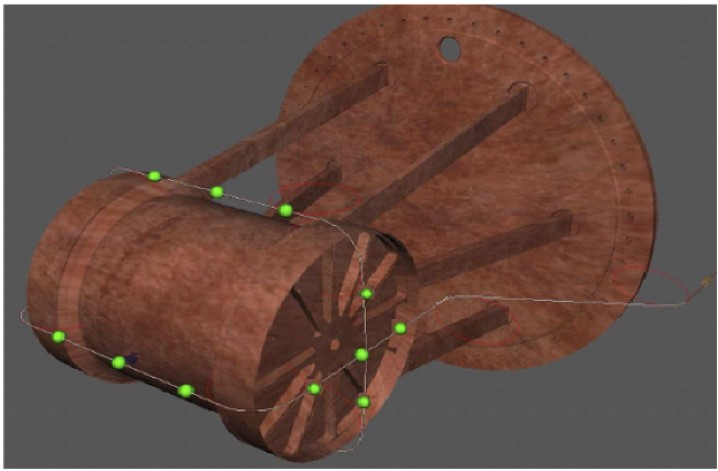
\includegraphics[keepaspectratio=true,width=\textwidth]{calibration_tube.jpg}
\end{center}
\renewcommand{\baselinestretch}{1}
\small\normalsize
\begin{quote}
\caption{A guide tube permits gamma sources to be inserted to known locations near the TPC.  Green dots indicate a few of the locations where the source may conventionally be placed.  Figure from~\cite{detectorPartI}.}
\label{fig:CalibrationGuideTube}
\end{quote}
\end{figure}
\renewcommand{\baselinestretch}{2}
\small\normalsize

The most critical type of calibration comes from external gamma sources.  The EXO experiment was constructed with a guide tube passing through the HFE-7000 refrigerant and wrapping loosely around the TPC, as shown in figure~\ref{fig:CalibrationGuideTube}.  Currently available to the experiment are sources containing $^{228}$Th (primary gamma line at $2615$ keV), $^{60}$Co (simultaneous emission of gammas at $1173$ and $1332$ keV), and $^{137}$Cs (gamma line at $662$ keV); additionally, a new $^{226}$Ra source became available in the summer of 2013 (numerous gammas, including $2448$ keV).  The $^{228}$Th and $^{60}$Co sources are available in weak and strong strengths, where the strong strength is chosen to produce a data rate that is still low enough that charge-light association can usually be done unambiguously.  Together these sources allow us to observe the detector response to external gammas with known energies, permitting energy calibrations, energy resolution measurements, and verification of Monte Carlo simulations.

All of these sources have been used periodically (roughly every three months) in calibration campaigns intended to permit a full characterization of the detector response across a wide energy range at a particular moment.  Additionally, the $^{228}$Th source has been deployed regularly, typically three times every week for $2-3$ hours, for the entire history of the dataset.  The richness of the accumulated $^{228}$Th source dataset, along with the benefit that it contains a relatively clean high-energy gamma line, make it particularly convenient to work with. It will play a prominent role in the generation of our lightmap described in chapter~\ref{ch:Lightmap}.

Other calibrations are also performed on the detector, and may in some instances supplement the information provided by the source data.  To perform direct calibrations of the APDs, one APD mount contains a light diffuser rather than an APD device; the diffuser can be illuminated by a laser through optical fibers~\cite{detectorPartI}.  The APDs can be calibrated by pulsing the laser while varying the voltages of the APDs to adjust their gain, and in this way it is possible to measure the gain of the APDs in situ.  A laser system was available at the beginning of the dataset used in this work; however, there were certain deficiencies to the laser system which made its data difficult to use, and as a result a new and more accurate laser system was commissioned in August 2012.  Laser data in some form has been collected roughly once per week for much of the time containing this dataset.  Composing the laser data into a coherent history of the APD gains is an ongoing project, but it has been possible to use APD gain information from specific moments to inform the APD noise model described in section~\ref{sec:DescriptionOfPhotonNoise}.

Just as it is possible and desirable to learn the gain of the APDs separately from other components using laser runs, it is also desirable to learn the relative gain of the electronics amplifiers separately from other detector function.  This is accomplished using ``internal calibrations'': simultaneously with software triggers solicited by the data acquisition, a switched capacitor injects charge into the input of the electronics cards of individual or groups of channels~\cite{EXOElectronicsFunctionalSpecification}.  The resulting waveform is then read normally, and the size of the output pulse reflects the gain of the electronics.  This system is employed approximately daily on all channels; it provides an excellent measure of relative changes in the electronics gains over time.  However, the absolute gains cannot be extracted accurately from this data due to variances in the capacitors, and must be obtained by other means.

To measure the absolute gains of the electronics, the front-end cards must be physically removed from their enclosures; when this is done, it is possible to use a more accurately calibrated capacitor to make an absolute gain measurement in the same style as the internal calibrations.  These ``external calibrations'' can be performed in two flavors: manual, in which a capacitor calibrated to $1\%$ is used to inject charge, and automatic, in which the calibration is automatically performed at a much faster rate but accuracy is limited to $2-3\%$.  Due to the inconvenience of removing electronics cards from their enclosures, this process has only been performed once in February 2011.  Both styles of external calibration were performed on the u-wire channels.  Less demanding needs for resolution on the v-wires and APD channels were foreseen, so only the less accurate automatic calibration was performed on those channels.  The data from these runs has not been fully analyzed, but may be revived in future analyses to permit a better calibrations of the subsequent internal calibrations which were taken.  A few electronics boards have been swapped since February 2011; channels on those boards will no longer have an absolute calibration available after the board swap, so it may be advisable to perform an additional external calibration~\cite{EnergyDocumentRun2a}.

\section{Summary}

This chapter has described some of the key characteristics of the construction and operation of the EXO-200 detector.  Background reduction has been a theme throughout -- EXO-200 has employed both passive and active methods to reject background and improve its sensitivity to $\beta\beta 0\nu$ decay.  Energy resolution has also been described as a key element in background rejection because the $2\sigma$ region of interest shrinks linearly with energy resolution, so with sufficiently precise energy measurements the rates of most backgrounds will decrease.  Chapter~\ref{ch:DenoisingTheory} will discusses a new scheme to extract more accurate energy measurements from the APD channels, thereby improving our overall energy resolution and the sensitivity of our $\beta\beta 0\nu$ half-life limit.
